\documentclass[a4paper, 20pt]{article}
\usepackage[english]{babel}
\usepackage{amsmath}
\usepackage{graphicx}
\usepackage{subcaption}
\usepackage{placeins}
\usepackage[T1]{fontenc}
\usepackage[utf8]{inputenc}
\usepackage{floatrow}
\usepackage{amsmath}

\author{Maarten de Jonge \\
    Inge Becht}
\date{\today}
\title{Assignment 4\\ 
Slammin' and Jammin'}

\begin{document}
\maketitle
\section{Introduction}
In this exercise the use of the fastSLAM algorithm is explored for the NXT
legorobot. The idea of this algorithm is that the robot makes a map using no a
priori knowledge of the environment,
while at the same time determining its position in the map.
To use SLAM in general, two types of data need to be extracted. Firstly, the robot needs to aqcuire landmarks from the
environment. These landsmarks in the case of this assignment are wall corners. To extract these
corners the same line extraction algorithm is used as in previous exercises (see assignment 2,3 and 4). 
Secondly, the robot needs odometry to measure its distance to map the information found by the
sensors correctly. This idea has been explored in a
previous exercise as well (see assignment 1), but uses a noise distribution to
make the next position given the previous one a certaint measure of uncertainty.

Although the outline of the SLAM algorithm is already given, the implementation
of both odometry and landmark detection were left open as an exercise. The next
section will show what was implemented. After this different experiments were
done witht he FastSLAM
algortihm to show what paramets can be of a decisive factor when working with a
particle filter.


\section{The implementation}
The implemention of the slam algorithm was given ready made in MATLAB code, and
can be run using the function \texttt{control\_panel.m}. The functions in
\texttt{FitLine.m} and \texttt{predict\_odo} still need to be completed.

\texttt{FitLine.m} is part of the implementation to find the landmarks for the
SLAM algorithm, and as the name suggests the idea is to fit a line given the
cluster of input points. First the x,y position of the centroid is found by
calculating the mean of the points in the cloud. The orientation of $\alpha$ (
We work in pool coordinates) depens on nom and denom, as given in the exercise.
Now $r$ can be decided using:

\begin{align*}
    r = x cos \alpha + y sin \alpha
\end{align*}

The x and y values used here are the centroid x and y calculated earlier.
Fitline now return the parameters $\alpha$ and $r$ for a possible line in the
point cloud.

. The file \texttt{predict\_odo} tries to predict the new position of the robot
given some uncertainty in the covariancy matrix and the sensor values in the
wheel.
The x and y positions are calculated as follows:

\begin{align*}
    x_{t+1} = x_{t} + dr_n * cos(dth_n + \theta_t)\\
    y_{t+1} = y_{t} + dr_n * sin(dth_n + \theta_t)\\
\theta_{t+1} = \left\{ \begin{array}{rl}
 \theta_t + \theta_d + -2*\pi &\mbox{ if $\theta_t + \theta_d > \pi$} \\
 \theta_t + \theta_d + 2*\pi&\mbox{ otherwise}
\end{array} \right.
\end{align*}
where $x_{t+1}$ is the $x$ position of a particle on time $t+1$, $dr_n$ is a noise
parameter that adds uncertainty in the amount of distance driven between each
timestep, $dth_n$ is noise parameter for $\theta$ and $\theta_d$ the
difference in theta value between $\theta_t$  and $\theta_{t+1}$.
Using the \texttt{TEST\_ODO.m} file a test can be made of the performance of the
odometry prediction. In \ref{fig:odo_test} the resulting image given this test
can be admired. Unfortunately there was baseline to test our results against,
except for the other students getting the same image as we did, as well as the
same value for the returned parameter \texttt{TOL\_JUMP} with a value of 10.5

\begin{figure}[!ht]
\centering
  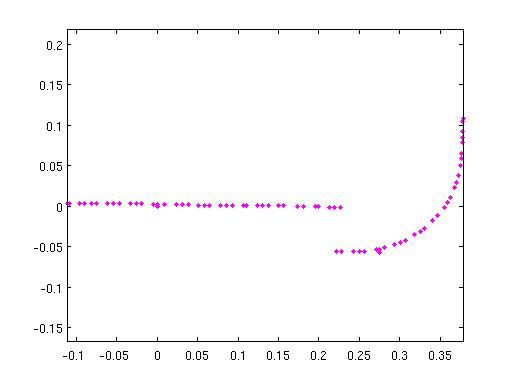
\includegraphics[width=0.5\textwidth]{Odo_test.jpg}
  \label{fig:odo_test}
  \caption{Figure represented byt the \texttt{ODO\_TEST.m} file. } 
\end{figure}


\section{Experiments}
Unfortunately we were unable to use the dataset recorded on the Mindstorms
robot, so all experiments were done on the provided sample logfile, in which the
robot moves forward for a bit through a hallway before turning left and
stopping.

\end{document}
